% mainfile: ../../../../master.tex
\subsection{cDNA quantification Nanodrop}
% The part of the label after the colon must match the file name. Otherwise,
% conditional compilation based on task labels does NOT work.
\label{task:20180116_cj1}
\tags{cdna,qnt,lab}
\authors{cj}
%\files{}
%\persons{}

\begin{figure}[H] % position of the figure 
    \centering
    \caption{Screenshots of the NanoDrop analysis of cDNA samples obtained after reverse transcription of the RNA extracted from bacterial cultures.}
    \label{fig:20180116_nanodrop}
    \begin{subfigure}[b]{0.49\textwidth}
        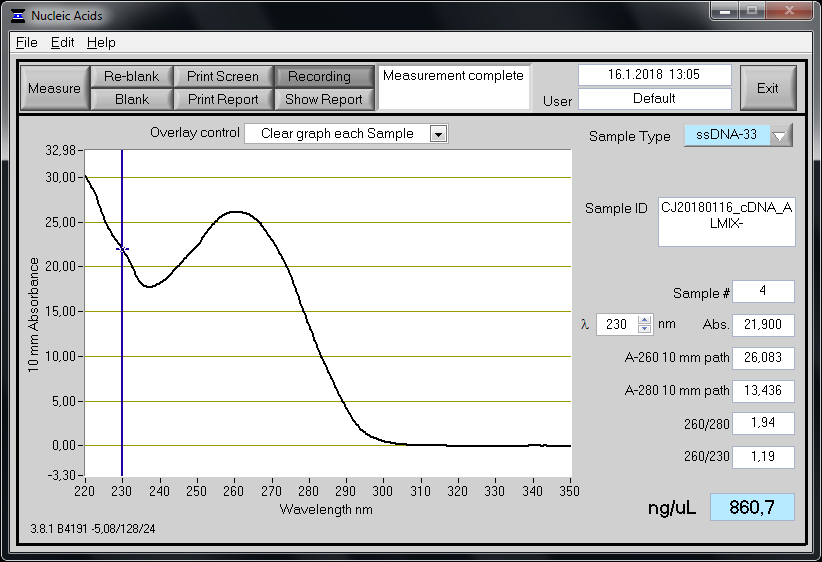
\includegraphics[width=\textwidth]{graphics/screenshots/CJ20180116_cDNA_ALMIX-.png}
        \caption{\texttt{cDNA ALMIX}}
        \label{sfig:CJ20180116_cDNA_ALMIX-}
    \end{subfigure}
    ~ 
    \begin{subfigure}[b]{0.49\textwidth}
        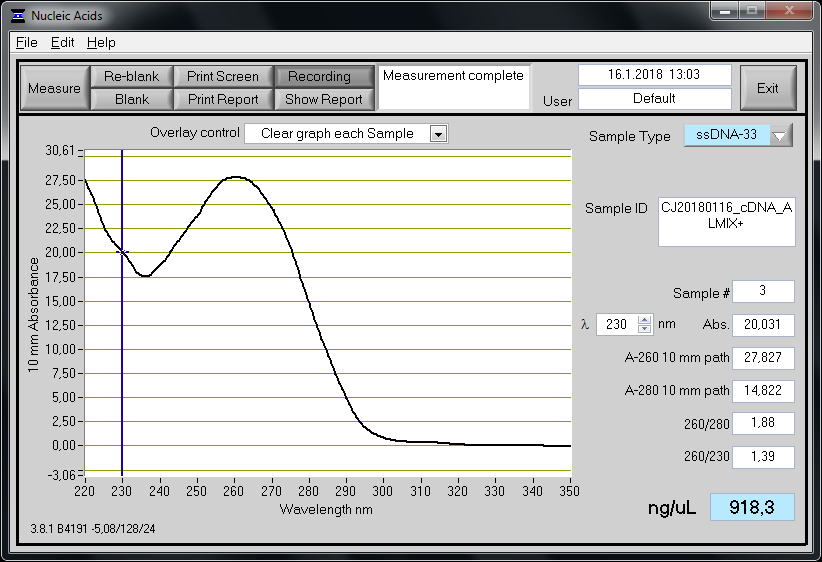
\includegraphics[width=\textwidth]{graphics/screenshots/CJ20180116_cDNA_ALMIX+.png}
        \caption{\texttt{cDNA ALMIX} negative control}
        \label{sfig:CJ20180116_cDNA_ALMIX+}
    \end{subfigure}
    \\
        \begin{subfigure}[b]{0.49\textwidth}
        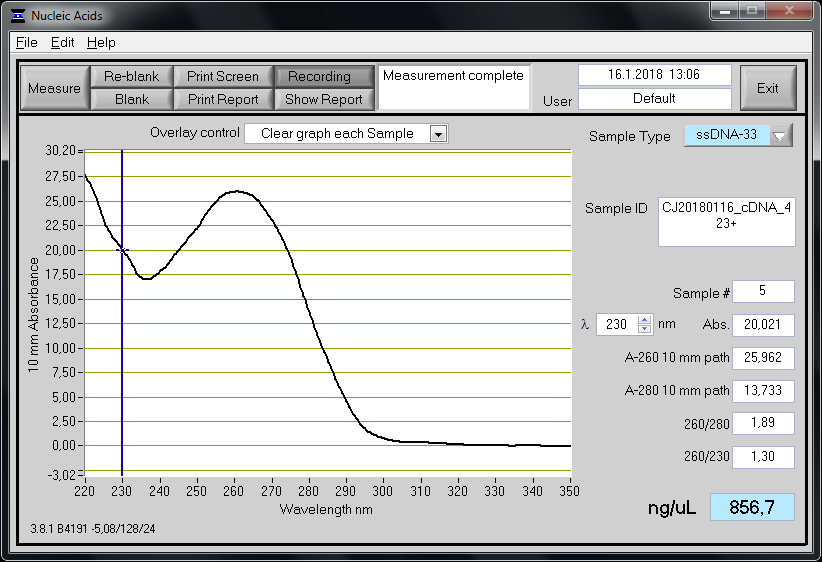
\includegraphics[width=\textwidth]{graphics/screenshots/CJ20180116_cDNA_423+.png}
        \caption{\texttt{cDNA 423}}
        \label{sfig:CJ20180116_cDNA_423+}
    \end{subfigure}
    ~ 
    \begin{subfigure}[b]{0.49\textwidth}
        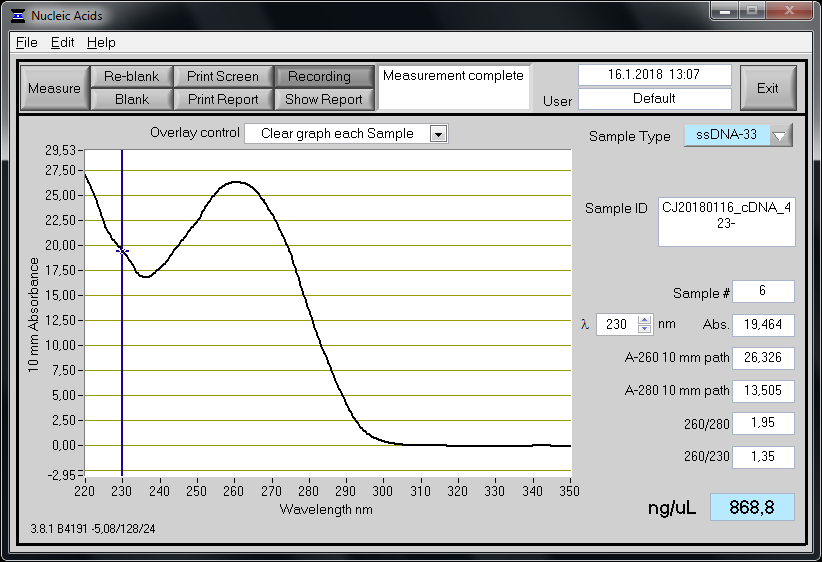
\includegraphics[width=\textwidth]{graphics/screenshots/CJ20180116_cDNA_423-.png}
        \caption{\texttt{cDNA 423} negative control}
        \label{sfig:CJ20180116_cDNA_423-}
    \end{subfigure}
    \\
        \begin{subfigure}[b]{0.49\textwidth}
        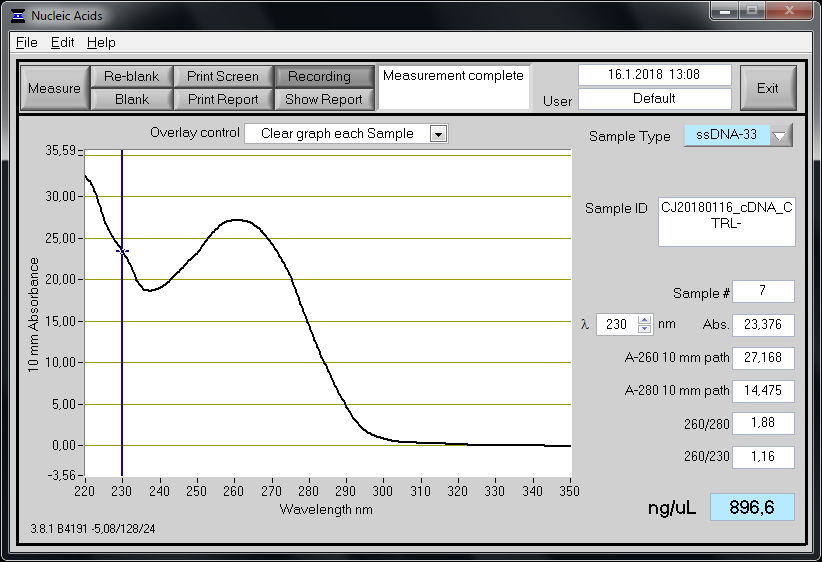
\includegraphics[width=\textwidth]{graphics/screenshots/CJ20180116_cDNA_CTRL-.png}
        \caption{\texttt{cDNA CTRL}}
        \label{sfig:CJ20180116_cDNA_CTRL-}
    \end{subfigure}
    ~ 
    \begin{subfigure}[b]{0.49\textwidth}
        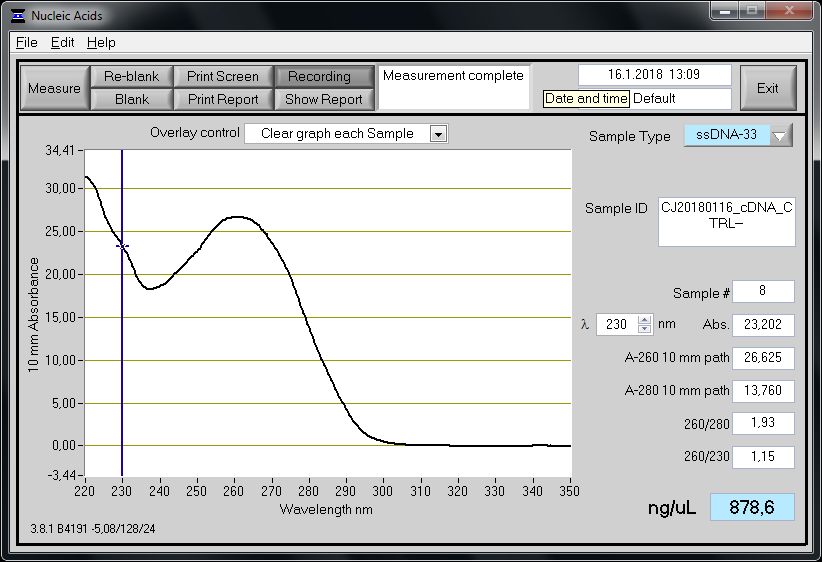
\includegraphics[width=\textwidth]{graphics/screenshots/CJ20180116_cDNA_CTRL--.png}
        \caption{\texttt{cDNA CTRL} negative control}
        \label{sfig:CJ20180116_cDNA_CTRL--}
    \end{subfigure}
\end{figure}



\begin{table}[htbp]
\caption{res/nanodrop/CJ20180116.txt}
\label{tab:CJ20180116}
\centering
\begin{tabular}{l l l l l l l l l l l l l }
\toprule
Sample ID & Time  & ng/ul  & A260  & A280  & 260/280  & 260/230  \\ \midrule
\texttt{CJ20180116\_BLANK\_H2O} & 13:02 & 0,50 & 0,015 & 0,004 & 4,00 & 0,27 \\
\texttt{CJ20180116\_cDNA\_ALMIX+} & 13:03 & 918,29 & 27,827 & 14,822 & 1,88 & 1,39 \\
\texttt{CJ20180116\_cDNA\_ALMIX-} & 13:04 & 860,74 & 26,083 & 13,436 & 1,94 & 1,19 \\
\texttt{CJ20180116\_cDNA\_423+} & 13:06 & 856,74 & 25,962 & 13,733 & 1,89 & 1,30 \\
\texttt{CJ20180116\_cDNA\_423-} & 13:07 & 868,77 & 26,326 & 13,505 & 1,95 & 1,35 \\
\texttt{CJ20180116\_cDNA\_CTRL-} & 13:08 & 896,56 & 27,168 & 14,475 & 1,88 & 1,16 \\
\texttt{CJ20180116\_cDNA\_CTRL--} & 13:09 & 878,64 & 26,625 & 13,760 & 1,93 & 1,15 \\

\bottomrule
\end{tabular}
\\
User: Default - Date: 16.1.2018 - Constant: 33,00 - Cursor position: 230 \
\end{table}
